\chapter{Synthesis}
\label{chap:synth}

The synthesis problem that we want attack requires a human model together with the local/remote devices. We will delay the environment discussion until the next section. Our framework can be shown pictorially in \figref{fig:genframe}. Here we assume that the human is watching a screen that 


\begin{figure}%
\centering
\begin{tikzpicture}[>=stealth]
\node [draw,circle,inner sep=2pt] (junc) at (-3cm,0) {};
\node [draw] at (-4.2cm,0cm) (H) {$H_u(\Delta)$};
\node [draw] (K) at (-1.5,-1) {K};
\node [draw] (Hp) at (-1.5,0) {$H_p$};
\node [draw,outer sep=0] (mr1) at (1,0) {$M_{r1}$};
\node [draw] (mr2) at (3,0) {$M_{r2}$};
\node [draw] (brain) at (-4,2) {$f(vision)$};
\draw[<-] (junc.south) node[below right] {$-$}|- (K.west) node[below,midway] {$\tau_l$};
\draw[<-] (H.west) -- ++(-0.5,0) node[above left] {$x_d$} -| ++(-0.5,2) -- (brain.west);
\draw[->] (H.east) -- (junc.west);
\draw[->] (junc.east) -- (Hp.west);
\fill [pattern = north east lines] (mr1.south west) rectangle ([yshift=-2mm]mr2.south east);
\draw[decorate,decoration={zigzag,pre length=0.2cm,post length=0.2cm,segment length=6}] (mr1.20) -- (mr2.160);
\draw[decoration={markings,  
  mark connection node=dmp,
  mark=at position 0.5 with 
  {
    \node (dmp) [inner sep=0pt,transform shape,rotate=-90,minimum width=5pt,minimum height=1.5pt,draw=none] {};
    \draw ($(dmp.north east)+(2pt,0)$) -- (dmp.south east) -- (dmp.south west) -- ($(dmp.north west)+(2pt,0)$);
    \draw ($(dmp.north)+(0,-2.5pt)$) -- ($(dmp.north)+(0,2.5pt)$);
  }
}, decorate] (mr1.-15) -- (mr2.-165);
\draw[->] (K.east) -| ([xshift=-5mm]mr1.west) node[midway,below] {$\tau_r$}-- (mr1.west);
\draw[<-] (mr2.east) -- ++(5mm,0) node[right] {$f_e$};
\draw[->] (Hp.east) -- ++(5mm,0) node[right] {$x_l$};
\draw[dashed,->] (mr2.north) |- (brain.east);
\draw[<-] (K.south) -- ++(0,-5mm) node[text width=3.5cm,below,align=center] {Various \\ Measurements};
\end{tikzpicture}
\caption{The general framework}%
\label{fig:genframe}%
\end{figure}


We start with the identified model \cite{fucavus} : The basic block diagram is given in \figref{fig:identifiedmodel}. The signal relations can be written as
\[
\pmatr{q\\x} = \bmatr{0 &W_{unc}\\H_{arm} & H_{arm}}\pmatr{p\\f}
\]

\begin{figure}%
\centering
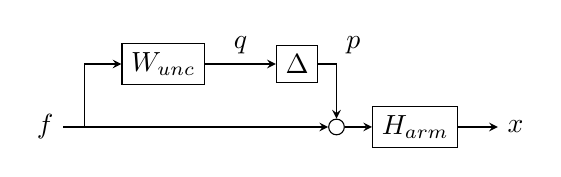
\begin{tikzpicture}[>=stealth]
\node at (-3.5cm,0) (f) {$f$};
\node [draw,circle,inner sep=2pt] (junc) at (0.2cm,0) {};
\node [draw] at (-2cm,0.8cm) (W) {$W_{unc}$};
\node [draw] at (-0.3cm,0.8cm) (delt) {$\Delta$};
\node [draw] at (1.2cm,0cm) (H) {$H_{arm}$};
\draw[->] (f) -- (junc.west);
\draw[->] (f) -- ++ (5mm,0) |- (W.west);
\draw[->] (W.east) -- (delt.west) node[midway,above] {$q$};
\draw[->] (delt.east) -| (junc.north) node[midway,above right] {$p$};
\draw[->] (junc.east) -- (H.west);
\draw[->] (H.east) -- ++(5mm,0) node[right] {$x$};
\end{tikzpicture}
\caption{The experimentally identified human model from \cite{fucavus}}%
\label{fig:identifiedmodel}%
\end{figure}

For our purposes we obtain a mapping from position to force via a partial inversion on the second channel. 
\[
\pmatr{q\\f} = \bmatr{-W_{unc} &W_{unc}\inv{H_{arm}}\\-1 &\inv{H_{arm}}}\pmatr{p\\x} = \bmatr{W_{unc}\\1}\bmatr{-1 &\inv{H_{arm}}}\pmatr{p\\x}
\]


\begin{figure}%
\centering

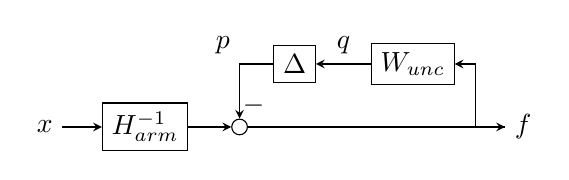
\begin{tikzpicture}[>=stealth]
\node at (0.6cm,0) (f) {$f$};
\node [draw,circle,inner sep=2pt] (junc) at (-3cm,0) {};
\node [draw] at (-0.8cm,0.8cm) (W) {$W_{unc}$};
\node [draw] at (-2.3cm,0.8cm) (delt) {$\Delta$};
\node [draw] at (-4.2cm,0cm) (H) {$H_{arm}^{-1}$};
\draw[<-] (H.west) -- ++(-0.5,0) node[left] {$x$};
\draw[->] (H.east) -- (junc.west);
\draw[->] (delt.west) -| node[midway,above left] {$p$} (junc.north) node[above right,inner sep=1pt] {$-$};
\draw[->] (W.west) -- (delt.east) node[midway,above] {$q$};
\draw[->] (junc.east) -- (f);
\draw[->] (f) -- ++(-0.6cm,0) |- (W.east);
\end{tikzpicture}
\caption{The mapping is inverted to obtain a model from position to force.}%
\label{fig:invidentifiedmodel}%
\end{figure}


The LTI transfer function $H$ is strictly proper hence its inverse is non-proper. Since we are only interested in the frequency response up to \SI{200}{\hertz} we use a low-pass filter on the position to tame the high frequency behavior. 
\[
W_{t} = \frac{4000}{s^2 + 280 s + 40000}
\]

After the application of this filter we obtain the overall human operator as
\[
\pmatr{q\\f} = \bmatr{W_{unc}\\1}\bmatr{-1 &\inv{H_{arm}}W_t}\pmatr{p\\x} = H_u \pmatr{p\\x}
\]
The next step is the obtain a local device model from force to position. We have selected the commercial PHANTOM device model which is identified in \cite{cavusfeygintendick}. The model is given by the following transfer function: 
\[
H_p = \frac{1}{s^2}\frac{s^2 + 5.716 s + 9.201\cdot 10^{4}}{(3.329\cdot 10^{-6} s^2 + 0.001226 s+1.536)}
\]


